\begin{question}
Using the function \texttt{randint} of the module \texttt{random} make a Monte Carlo simulation of rolling three dice to check the probability of getting the same values on the three of them.
From probability theory you should expect:

\[P_{d1=d2=d3} = \frac{1}{6}\cdot\frac{1}{6}\cdot\frac{1}{6}\cdot 6 = \frac{1}{36} = 0.0278\]
\end{question}

\cprotEnv\begin{solution}
\begin{ipython}
from random import seed, randint

seed(1)
trials = 10000000
success = 0

for _ in range(trials):
    d1, d2, d3 = randint(1, 6), randint(1, 6), randint(1, 6)
    if d1 == d2 and d2 == d3:
        success += 1

print ("The probability to get three equal dice is {:.4f}".format(success/trials))
\end{ipython}
\begin{ioutput}
The probability to get three equal dice is 0.0278
\end{ioutput}
\end{solution}

\begin{question}
Two fair dice are rolled, find the probability that their sum is:
\begin{enumerate}[start=1]
	\item equal to 1;
	\item equal to 4;
	\item less than 13.
\end{enumerate}
	
\noindent\textbf{Hint:} the possible combinations of the outcomes of two dice are 36 (to realize it you can simply think that for each one of the six faces of the first die you have six possible faces of the second hence $6\cdot 6=36$). It is not possible to get 1 since the dice have no face with 0 so the first probability should come out 0. The sum of the two dice is always less than 13 (the maximum is 12\ldots) so the answer to point 3 is 1. We can get a sum of 4 in 3 cases (1-3, 3-1 or 2-2) so the expected probability is $3/36=1/12=0.0833$
\end{question}

\cprotEnv\begin{solution}
\begin{ipython}
import random

random.seed(1)
successes = {"=1":0.0, "=4":0.0, "<13":0.0}
trials = 100000

for _ in range(trials):
    d1 = random.randint(1, 6)
    d2 = random.randint(1, 6)

    if (d1 + d2) == 1:
        successes["=0"] += 1.0
    if (d1 + d2) == 4:
        successes["=4"] += 1.0
    if (d1 + d2) < 13:
        successes["<13"] += 1.0

for k,v in successes.items():
    print ("P({}): {:.3f}".format(k, v/trials))
\end{ipython}
\begin{ioutput}
P(=1): 0.000
P(=4): 0.084
P(<13): 1.000
\end{ioutput}
\end{solution}

\begin{question}
Write a Greedy Pig (see Ex.~\ref{ex:greedy_pig}) Monte Carlo simulation for a player aiming at $k$ points each turn (i.e. the turn simulation goes on until a 1 is rolled or $k$ points are reached).

Plot the distribution of the average number of points as a function of $k$.
\end{question}
\cprotEnv\begin{solution}
\begin{ipython}
import numpy as np
from random import randint

k = 20
sim = 1000000
points = [0 for _ in range(51)]

for s in range(sim):
    for k in range(1, 51):
        p = 0 
        while p < k:
            d = randint(1, 6)
            if d == 1:
                p = 0
                break
            else:
                p += d

points[k] += p
points = np.array(points)/sim
\end{ipython}

Figure~\ref{fig:greedy_pig_sim} confirms what has been already found in a previous Exercise. Aiming at 20 points per turn is the strategy that maximizes the number of expected points.

\begin{figure}[htbp]
	\begin{center}
		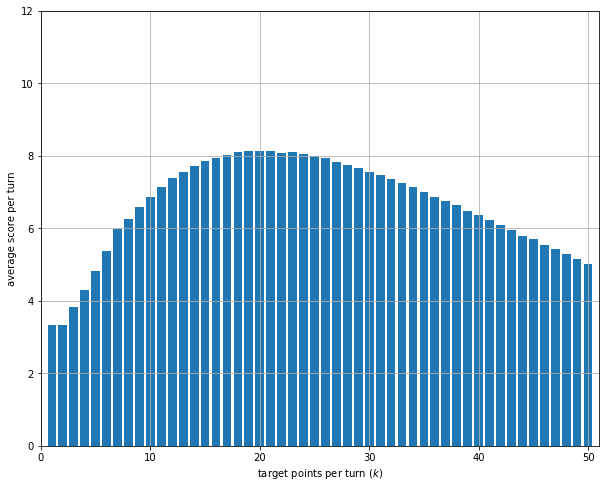
\includegraphics[width=0.7\linewidth]{figures/greedy_pig_sim}
	\end{center}
\caption{Distribution of expected number of points per turn.}
\label{fig:greedy_pig_sim}
\end{figure}
\end{solution}

\begin{question}
There are 60 chemical flasks in the laboratory, 6 of which are incorrectly labeled. What is the chance that if we randomly choose 5 flasks, exactly 3 of them will be labeled correctly ?

\noindent\textbf{Hint:} the probability is approximately 0.5 \%.
\end{question}

\cprotEnv\begin{solution}
\begin{ipython}
import random

flasks = ["C"]*54 + ["U"] * 6
random.seed(1)
trials = 1000
success = 0.

for _ in range(trials):
    draw = random.sample(flasks, 5)
    if draw.count("U") == 3:
        success += 1.

print ("Probability: {:.3f}%".format(success/float(trials)*100))
\end{ipython}
\begin{ioutput}
Probability: 0.499%
\end{ioutput}
\end{solution}

\begin{question}
Given the following historical series (1895-2020) find average September temperature in US and report the 99\% confidence interval of your measure.
\noindent
Input (temperatures are in Fahrenheit degrees): \href{https://raw.githubusercontent.com/matteosan1/finance_course/develop/libro/input_files/histo_temp.csv}{histo\_temp.csv}
\end{question}

\cprotEnv\begin{solution}
\begin{ipython}
from scipy.stats import norm
import numpy as np
import pandas as pd

# first download the input file
df = pd.read.csv("histo_temp.csv")
temperatures = df['T'].to_array()
alpha = 0.99

A = norm.ppf((1 + alpha)/2)
m, se = np.mean(temperatures), np.std(temperatures)
h = A*se/np.sqrt(len(temperatures))

print ("Avg temperature in September (US): {:.1f}".format(m))
print ("{:.1f}% confidence interval: +- {}".format(alpha*100, h))
\end{ipython}
\begin{ioutput}
Avg temperature in September (US): 65.1
99% confidence interval: +- 0.3
\end{ioutput}
\end{solution}

%\begin{question}
%Using the function \texttt{normal} of \texttt{numpy.random} simulate the price of a stock which evolves according to a log-normal stochastic process with a daily rate of return \(\mu=0.1\) and a volatility \(\sigma=0.15\) for 30 days.
%Also plot the price. Try to play with \(\mu\) and \(\sigma\) to see how the plot changes.
%\end{question}
%
%\cprotEnv\begin{solution}
%\begin{ipython}
%from numpy.random import normal, seed
%from matplotlib import pyplot as plt
%import math
%
%S = 100
%mu = 0.1
%sigma = 0.15
%T = 1
%seed(1)
%
%historical_series = [S]
%for i in range(30):
%    S = S * math.exp((mu - 0.5 * sigma * sigma) * T +
%        sigma * math.sqrt(T) * normal())
%    historical_series.append(S)
%
%plt.plot(range(31), historical_series)
%plt.xlabel("days")
%plt.ylabel("Price of stock X")
%plt.show()
%\end{ipython}
%
%\begin{figure}[!htb]
%\begin{center}
%  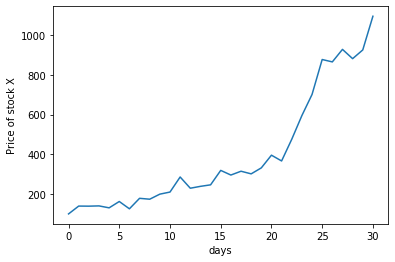
\includegraphics[width=0.7\linewidth]{figures/lesson6_solutions_5_0.png}
%\end{center}
%\caption{A realization of a stock price 30 days evolution.} 
%\end{figure}
%\end{solution}
